%!TEX root = spadini_davide.tex

\chapter{Implementation}
\label{cha:implementation}
Using WebRTC as ``network handler'' gave us the possibility to avoid the manual management of some events (e.g. the failure of a node, the retransmission of a message, etc. etc.), because they are directly handled by it. In the previous sections we saw how the Google WebRTC APIs work and the algorithm details, however in order to combine them to work properly we have to take care of mechanisms that are not mentioned in the original paper of the algorithm nor covered in their implementation. The most important one is how the nodes can exchange their EasyRTC identifiers, but we also discuss some improvements that we achieved using WebRTC.

\section{Tracker}
\label{cha:tracker}
In Sect.~\ref{cha:webrtc} we saw how a node can initialize a connection to another node using the EasyRTC Framework: at the beginning they both have to contact the EasyRTC Server to obtain the ID, and then pass the identifier of the other node to the \textsf{\textit{connect}} function in order to establish the connection. However, EasyRTC does not specify how the nodes have to exchange these identifiers: for this purpose we created a tracker. 

When the nodes bootstrap, they have to contact the EasyRTC Server in order to join the network and then they have to register themselves to the tracker. In this way the latter will eventually have the complete list of the nodes present in the network. When a peer needs to connect to another one (i.e. to replace a broken link):
\begin{itemize}
	\item it asks the tracker a reference of a new node
	\item the tracker chooses an ID at random from the list and it returns it to the peer
	\item the peer analyzes the answer and connects to that ID
\end{itemize}

We use the tracker to provide all nodes with a list of ``initial peers'' to contact in order to start the algorithm (more information in Sect.~\ref{cha:wormhole}), to replace the broken links and for all the necessary replacements expected from the algorithm. The main tasks of the tracker are shown in Fig.~\ref{fig:tracker}.

In this project the tracker acts like a central server: we only have one tracker for all the nodes, and it has to handle and serve all the requests that derive from the nodes. However, this is not a problem since it has relatively low load (the link replacements are rare) and the algorithm is designed to reduce the number of new network connections created. 

The tracker is hosted on Heroku\footnote{Heroku is a cloud platform that lets companies build, deliver, monitor and scale apps \url{https://www.heroku.com/}} and is implemented in Node.js. The nodes contact the tracker using \textsf{XMLHttpRequest} (XHR)\footnote{XMLHttpRequest is an API available to web browser scripting languages such as JavaScript that is used to send HTTP or HTTPS requests to a web server and load the server response data back into the script} and then they parse the response to obtain what they asked.

\begin{figure}[ht]
  \centering
  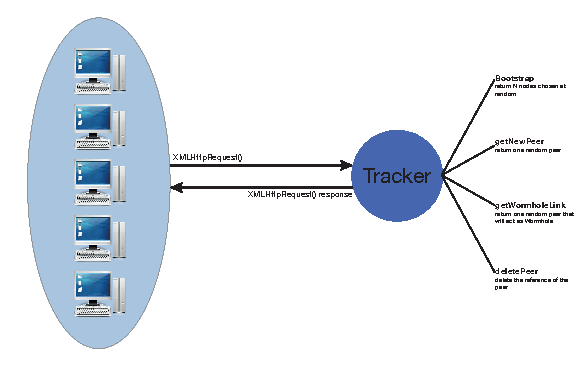
\includegraphics[keepaspectratio=true, width=0.8\textwidth]{images/tracker}\caption{The main tasks of the tracker}
  \label{fig:tracker}
\end{figure}

\section{Project Environment}
\label{cha:design}
We implemented and tested the project in a real environment and also in simulation. WebRTC APIs are web browser APIs, meaning that they can only work in a browser session. So we developed a first version of the \ac{WPSS} that works in the browser, and tested it with few nodes (100) using Google Chrome\footnote{Google Chrome is a free-ware web browser developed by Google} as browser. Then, in order to test it in a bigger environment we used a simulator. Both versions are implemented using the framework \textbf{Hivejs-Framework} provided by the creator of the algorithm, the Hive Streaming\footnote{Hive Streaming provides network solutions for media distribution and performance analysis. Started as a spin-off in 2007 from the Swedish Institute for Computer Science and the Royal Institute of Technology in Stockholm, the company maintains a strong focus on research and development. \url{https://www.hivestreaming.com}} company. This framework is written in Typescript\footnote{TypeScript is a typed superset of JavaScript that compiles to plain JavaScript. \url{http://www.typescriptlang.org}}, and it enables us to choose if we want to run the project on browser or directly in Node.js simulating a lot of instances. 

At bootstrap-time, all the nodes contact the EasyRTC Server (Sect.~\ref{subsec:easyrtc_server}) to join the network. Then, they need a way to build the base overlay with a fixed number of nodes, so they have to register themselves to the tracker, which it will return the list of the nodes that they have to contact. The tracker is also used to replace the broken links with new ones. In all the other cases, the peers communicate between each other without the help of an external server. The schema with all the steps is shown in Fig.~\ref{fig:project_architecture}.

\begin{figure}[ht]
  \centering
  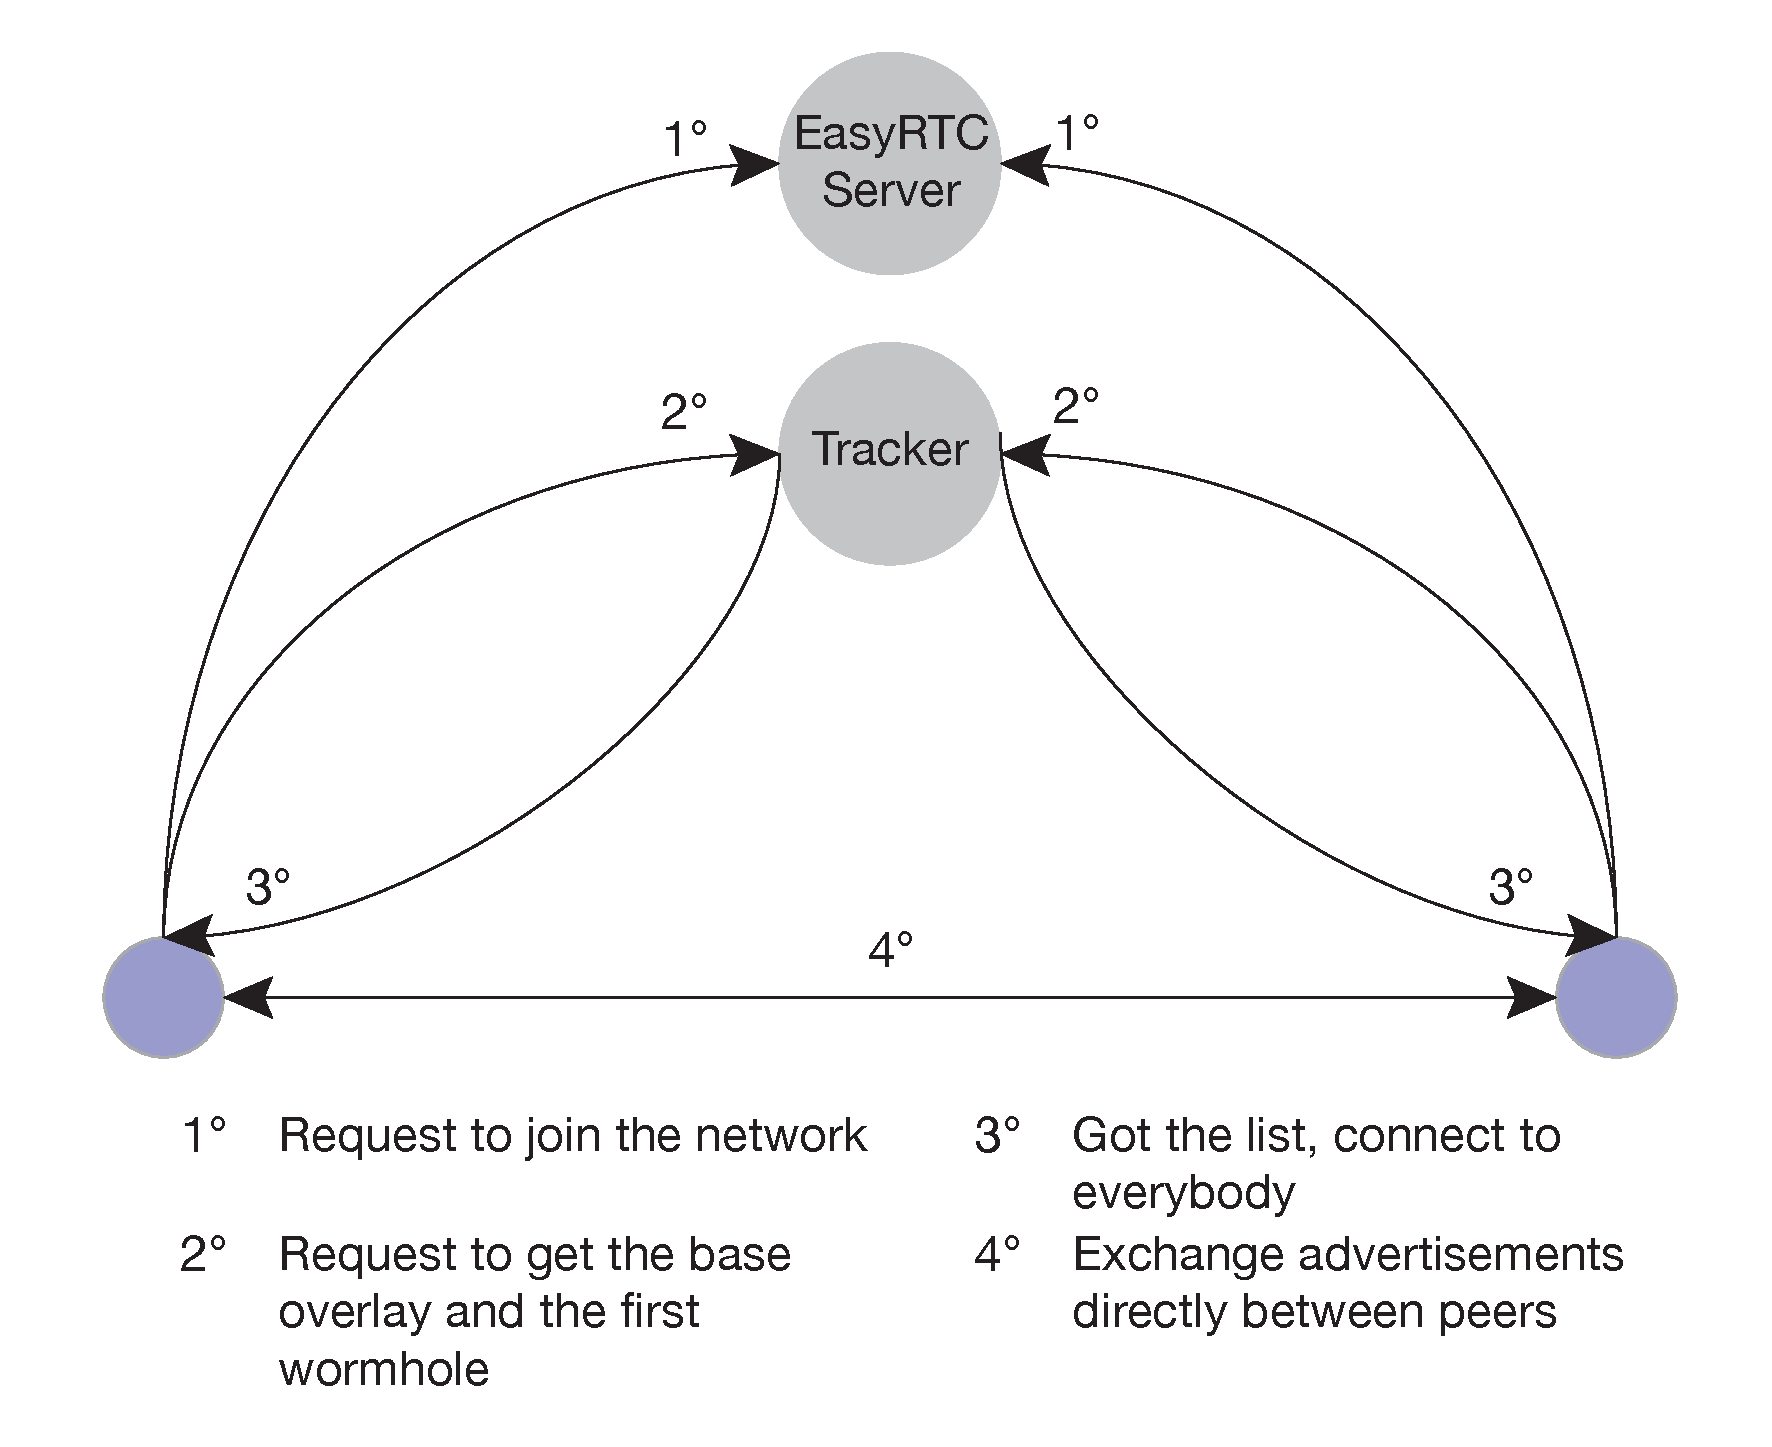
\includegraphics[keepaspectratio=true, width=0.8\textwidth]{images/project_architecture}\caption{The architecture of the project, with the initial steps the nodes have to accomplish}
  \label{fig:project_architecture}
\end{figure}


\section{Node.js Modules}
\label{sec:modules}
The Hivejs-Framework has a WebRTC module for handling peer-to-peer connections which, as explained in Sect.~\ref{sec:easy_tc}, is EasyRTC. Then we used a lot of other modules, the most important ones are:

\begin{itemize}
	\item \textbf{Browserify}: with browserify we can use some core Node.js modules and many of the thousands modules on npm in our browser-side code
	\item \textbf{Grunt}: it is a task runner, we use it to compile, optimize and ``browserify'' our code. More information at \url{http://gruntjs.com}
	\item \textbf{Inversify}: Inversify is a lightweight (4KB) pico inversion of control (IoC) container for TypeScript and JavaScript applications
	\item \textbf{Q}: a library for promises, more information at \url{https://www.npmjs.com/package/q}
	\item \textbf{Fs}: we use this module only in simulation to write and save the logs of the nodes on local files.
\end{itemize}

The project in order to work correctly needs Node.js version 0.12.5, npm version 2.11.2 and Typescript version 1.7.3.

\section{Special Tools}
We used a lot of tools to simplify the testing phase but also the implementation. One of the most important is NetworkX\footnote{\url{https://networkx.github.io}}, a Python language software package for the creation, manipulation, and study of the structure of complex networks. We used this tool to periodically draw the graphs of the network, in order to have a better representation of the overlays and to check the correctness of the implementation. 


\section{Possible improvements}
\label{sec:improvements}
In Sect.~\ref{cha:wormhole} we saw that when a node has to forward a sample it uses the \getMetropolisHastingsNeighbour function. In order to be sure that the message will be sent correctly, they use this function over the stable base overlay. In fact, while the wormhole overlay will be in constant change, their implementation uses a failure detector to replace the broken links in the base overlay, keeping constant the degree of the nodes. Using WebRTC instead we eliminate the failure detector, because this part is handled by the EasyRTC Framework. In this way what we obtain is that both the overlays are more stable, and this enables us to use the \getMetropolisHastingsNeighbour over all the connected peers, not only over the base overlay. This principle benefits the average hop count, which is the average number of hops a sample will have to take in order to be consumed from some other nodes. This is due to the fact that the peer will have to choose to whom send the sample from a bigger set, so the probability that the chosen node will already have the sample decreases. We will see in Sect.~\ref{cha:evaluation} that also in presence of churn our implementation keeps lower the average hop count. In addition to this we do not have other benefits using WebRTC. 

Another little changing that we made is in the \acceptAd method: it makes sure that every node consumes advertisements at the same rate, namely one advertisement in each $\Delta$ time period. In the original paper in order to control the rate they approximate the period of receiving advertisements. In our implementation instead we check only if the node has already accepted a sample in the current period, otherwise it consumes it. We will see in a specific test that our \acceptAd method successfully balances advertisements over public and private nodes.
